\newcommand\UniversiteAdi{Niğde Ömer Halisdemir Üniversitesi}
\newcommand\BolumAdi{MEKATRONİK BÖLÜMÜ}
\newcommand\DersKodu{MKT2002}
\newcommand\DersAdi{BİLGİSAYARLI KONTROL SİSTEMLERİ}
\newcommand\SinavAdi{Ara Sınav}
\newcommand\SinavTarihi{10.03.2025}
\newcommand\SinavSaati{10:00}
\newcommand\SinavSuresi{90dk}

\pagestyle{fancy}
\fancyhf{} % clear existing header/footer entries
\fancyhead[R]{Öğrenci No:\hspace{4.5cm}}
\fancyhead[L]{Ad Soyad:\hspace{7cm}}
\noindent
\begin{tabular}{
    p{0.15\linewidth}
    p{0.15\linewidth}
    p{0.3\linewidth}
    p{0.1\linewidth}
    p{0.15\linewidth}}
    \multicolumn{5}{c}{\textbf{\BolumAdi}}\\
    \multicolumn{5}{c}{\textbf{\DersAdi}}\\\hline
    \multicolumn{1}{|r|}{Ders Kodu:}&
    \multicolumn{1}{|c|}{\DersKodu}&
    \multicolumn{1}{|c|}{}& 
    \multicolumn{1}{|r|}{Tarih:}&
    \multicolumn{1}{|c|}{\SinavTarihi} \\\hline
    \multicolumn{1}{|r|}{Sınav Türü:}&
    \multicolumn{1}{|c|}{\SinavAdi}&  
    \multicolumn{1}{|c|}{}&
    \multicolumn{1}{|r|}{Saat:}&
    \multicolumn{1}{|c|}{\SinavSaati}\\\hline
    \multicolumn{1}{|r|}{Dönemi:}&
    \multicolumn{1}{|c|}{2024-2025}&
    \multicolumn{1}{|c|}{}&
    \multicolumn{1}{|r|}{Süre:}&
    \multicolumn{1}{|c|}{\SinavSuresi} \\\hline
    &&&&\\
\end{tabular}\\\\
\noindent\begin{center}
\begin{tabular}{|r|c|c|c|c|c|}\hline
    \textbf{Soru:}&
    \textbf{1a}&
    \textbf{1b}&
    \textbf{2a}&
    \textbf{2b}&
    \textbf{Toplam}\\\hline
    \textbf{Puan:}&
    \textbf{25}&
    \textbf{25}&
    \textbf{25}&
    \textbf{25}&
    \textbf{100}\\\hline
    \textbf{Not:}&25&25&25&25&100\\\hline
\end{tabular}\end{center}
\noindent\textbf{Uyarı:}
\begin{itemize}\bfseries
    \item Soruları dikkatlice okuyunuz. Hesap makinesi kullanılabilir.
    \item Defter, kitap ve notlar açık bir sınavdır.
    \item İşlemleri atlamadan ve ayrıntılı olarak veriniz. Sadece nümerik yanıtlar veya çizimler ara işlemler olmadan kabul edilmemektedir.
    \item Yuvarlamalar 2 hane yapılacaktır. $\mathbf{1.99456\approx1.99}$ olarak alınacaktır.
\end{itemize}

\begin{enumerate}[\bfseries S1.]
    \item İkinci dereceden bir sistem
    \begin{equation}
        G(s)=\frac{12}{s^2+5s+4}
    \end{equation}
    olarak verilmiştir.
    \begin{enumerate}
        \item(25p)\,$G(s)$ transfer fonksiyonunun z tanım bölgesinde karşılığını $G(z)$'yi elde ediniz. 
        Dönüşüm,
        \begin{equation}
            G(z)=\mathcal{Z}\left\{(1-e^{-sT})\left(\frac{12}{s(s^2+5s+4)}\right)\right\}
        \end{equation}
        olmak üzere verilen transfer fonksiyonu
        \begin{equation}
        \begin{split}
            \frac{12}{s^3+5s^2+4s}&=\frac{A}{s}+\frac{B}{s+1}+\frac{C}{s+4}\\
            &=\frac{As^2+5As+4A+Bs^2+4Bs++Cs^2+Cs}{s(s+1)(s+4)}\\
            As^2+5As+4A+Bs^2+4Bs++Cs^2+Cs&=12\\
            A+B+C=0\,&\,5A+4B+C=0\,4A=12\\
            A=3\,&\,B=-4\,C=1\\
            \frac{12}{s^3+5s^2+4s}&=\frac{3}{s}-\frac{4}{s+1}+\frac{1}{s+4}
        \end{split}
        \end{equation}
        olarak parçalanır. Bu durumda
        \begin{equation}
        \begin{split}
            G(z)&=\mathcal{Z}\left\{(1-e^{-sT})\left(\frac{3}{s}-\frac{4}{s+1}+\frac{1}{s+4}\right)\right\}\\
            &=\left(1-z^{-1}\right)\left(\mathcal{Z}\left\{\frac{3}{s}\right\}-\mathcal{Z}\left\{\frac{4}{s+1}\right\}+\mathcal{Z}\left\{\frac{1}{s+4}\right\}\right)\\
            &=\left(\frac{z-1}{z}\right)\left(\frac{3z}{z-1}-\frac{4z}{z-e^{-1}}+\frac{z}{z-e^{-4}}\right)\\
            &=\frac{(3+e^{-4}-4e^{-1})z+(e^{-1}+3e^{-5}-4e^{-4})}{z^2-(e^{-1}+e^{-4})z-e^{-5}}\\
            &=\frac{1.55z+0.31}{z^2-0.39z+0.01}
        \end{split}
        \end{equation}
        elde edilir.

        \item(25p)\,$G(z)$ transfer fonksiyonu için fark denklemini elde ediniz. 
        Elde edilen ifadeden yola çıkılarak fark denklemi
        \begin{equation}
            \begin{split}
                G(z)&=\frac{1.55z+0.31}{z^2-0.39z+0.01}\\
                \frac{y(k)}{u(k)}&=\frac{1.55z+0.31}{z^2-0.39z+0.01}\\
                (z^2-0.39z+0.01)y(k)&=(1.55z+0.31)u(k)\\
                (1-0.39z^{-1}+0.01z^{-2})y(k)&=(1.55z^{-1}+0.31z^{-2})u(k)\\
                y(k)-0.39z^{-1}y(k)+0.01z^{-2}y(k)&=1.55z^{-1}u(k)+0.31z^{-2}u(k)\\
                y(k)-0.39y(k-1)+0.01y(k-2)&=1.55u(k-1)+0.31u(k-2)\\
                y(k)&=0.39y(k-1)-0.01y(k-2)+1.55u(k-1)+0.31u(k-2)
            \end{split}
        \end{equation}
        olarak hesaplanır.      
    \end{enumerate}
    \item Zaman isterleri $t_s=2\,s$ ve aşım $\%20$ ve örnekleme zamanı $T=0.5\,s$ olarak verilmiştir. 
    \begin{enumerate}
        \item(25p)\,Kutupların konumunu z tanım bölgesinde elde ediniz ve z tanım bölgesinde çiziniz. 
        Aşım kriterinden
        \begin{equation}
        \begin{split}
            \zeta&=\frac{log(0.2)}{\sqrt{\pi^2+log(0.2)^2}}\\
            &=0.46
        \end{split}
        \end{equation}
        ve yerleşme zamanından ise 
        \begin{equation}
            \begin{split}
                w_n&=\frac{4}{t_s\zeta}\\
                &=\frac{4}{2\cdot 0.45595}\\
                &=4.39
            \end{split}
        \end{equation}
        elde edilir. S tanım bölgesinde kutuplar
        \begin{equation}
            s=-2\pm3.90i
        \end{equation}
        olarak tanımlanır. Z tanım bölgesine geçiş $z=e^{sT}$ ile yapılır ve z tanım bölgesinde kutuplar
        \begin{equation}
            \begin{split}
                z&=e^{0.5(-2\pm3.90i)}\\
                z&=e^{-1\pm1.95i}\\
                z&=e^{-1}\phase{\pm1.95}\\
                z&=0.37\phase{\pm111.73^o}\\
                z&=-0.14\pm0.34i
            \end{split}
        \end{equation}
        olarak elde edilir.
            
        \begin{center}
        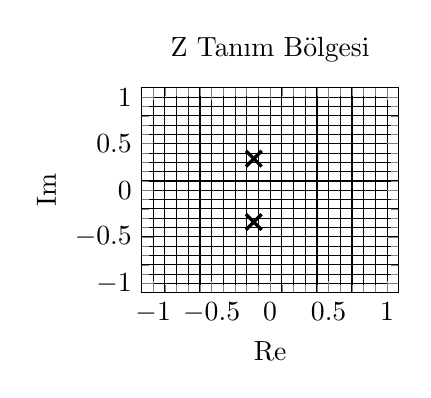
\begin{tikzpicture}
            \begin{axis}[samples=500,domain=-1.1:1.1,,minor tick num=4,restrict y to domain =-1.1:1.1,xmin=-1.1,xmax=1.1,ymin=-1.1,ymax=1.1,xlabel={Re},ylabel={Im},title={Z Tanım Bölgesi},grid=both,minor grid style={color=black},major grid style={color=black},width=0.4\textwidth]
                \draw (axis cs: 0, 0) circle [radius=100];
                \addplot[mark=x,only marks,mark color=black,mark size=4pt,very thick] coordinates {(-0.14,0.34) (-0.14,-0.34)};
            \end{axis} 
        \end{tikzpicture}  
        \end{center}

        \item(25p)\, Z tanım bölgesinde elde edilen kutuplara sahip polinom $p(z)$ olmak üzere
        \begin{equation}
            G(z)=\frac{1}{p(z)}
        \end{equation}
        olarak tanımlanan $G(z)$ transfer fonksiyonuna karşılık düşen fark denklemini elde ederek $0\leq t\leq 2$ aralığında birim basamak yanıtını hesaplayınız ve yaklaşık olarak çiziniz. 
        Transfer fonksiyonu
        \begin{equation}
        \begin{split}
            G(z)&=\frac{1}{(z+0.14+0.34i)(z+0.14-0.34i)}\\
            &=\frac{1}{z^2+0.28z+0.14}
        \end{split}
        \end{equation}
        olarak elde edilir. Fark denklemi ise 
        \begin{equation}
            \begin{split}
                \frac{y(k)}{u(k)}&=\frac{1}{z^2+0.28z+0.14}\\
                (z^2+0.28z+0.14)y(k)&=u(k)\\
                (1+0.28z^{-1}+0.14z^{-2})y(k)&=z^{-2}u(k)\\
                y(k)+0.28z^{-1}y(k)+0.14z^{-2}y(k)&=z^{-2}u(k)\\
                y(k)+0.28y(k-1)+0.14y(k-2)&=u(k-2)\\
                y(k)&=-0.28y(k-1)-0.14y(k-2)+u(k-2)
            \end{split}
        \end{equation}
        şeklindedir.

        \begin{center}
        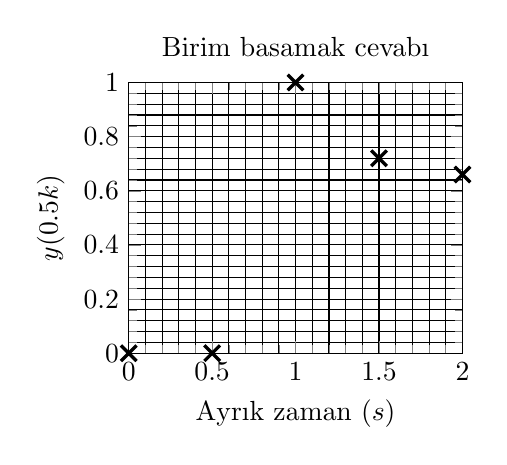
\begin{tikzpicture}
        \begin{axis}[samples=500,domain=0:2,,minor tick num=4,restrict y to domain =0:1,xmin=0,xmax=2,ymin=0,ymax=1,xlabel={Ayrık zaman $(s)$},ylabel={$y(0.5k)$},title={Birim basamak cevabı},grid=both,minor grid style={color=black},major grid style={color=black},width=0.48\textwidth]
            \addplot[mark=x,only marks,mark color=black,mark size=4pt,very thick] coordinates {(0,0) (0.5,0) (1,1) (1.5,0.72) (2,0.66)};
        \end{axis} 
        \end{tikzpicture}  
        \end{center}
    \end{enumerate}
    

\end{enumerate}
